\chapter{関連研究・技術}
 
\section{関連研究}

\subsection{DDoS攻撃を行うマルウェアの分析}
DDoS攻撃を行うIoTデバイスを対象としたマルウェアの分析を行った研究が行われている.組込みシステム向けマルウェアMiraiの攻撃性能評価\cite{攻撃性能評価を行った研究}では,MiraiをVM上で動作させ通信の様子や攻撃の流れの動作を確認し,攻撃性能を計測した.実機実験として,ローカルネットワーク上で複数の組み込みボード(odroid-c2)を用いてVMと同様にMiraiの動作環境を構築し,攻撃性能の影響の調査を行った.組み込みシステム向けTCP/IPスタックからなるhttpサーバーが動作する静的な組込みシステムのプロトタイプを対象に攻撃を行い,DDoS攻撃時にはCPU使用率が大幅に上がることを明らかにした.しかし,研究結果からマルウェアに対して具体的な検知手法の提案がなされていない.
%IoT機器へのTelnetを用いたサイバー攻撃の分析では,
IoTマルウェアによるDDos攻撃の動的解析による観測と分析\cite{観測と分析}では,ハニーポットを用いて収集したIoTマルウェアの検体を用いてARM,MIPS,MIPSELの3種類のCPUアーキテクチャを用いてマルウェアを動作させその挙動を観測し,ダミーC\&Cサーバーを用いて攻撃再現実験を行いDoS攻撃の観測を行った.マルウェアに対してDoS攻撃命令が届くタイミングは各感染ホストによって様々であり,マルウェアの動作直後に集中されるわけではないことがわかった.このことから,動的解析によりDoS攻撃の命令の挙動を観測する場合には,長期的な観測が必要になる.

%\sbusection{動的解析を用いたマルウェア検知の研究}
\subsection{動的解析を行ったマルウェア検知の研究} % subsectionのタイトル

マルウェアの検知手法として,APIを特徴として用いた研究が広く行われている.
API呼び出しとそれに伴う経過時間とシステム負荷を用いた検知手法\cite{パターン}では,API呼び出しパターン,API呼び出しによる経過時間とシステム負荷を特徴量としたマルウェア検知手法を提案した.マルウェア1検体あたりに10秒間動作をさせ,その間に得られた動的解析ログからAPI呼び出しとそれに伴う経過時間とメモリ使用量の情報を抽出し,マルウェアの特徴抽出を行い,機械学習アルゴリズムを用いてマルウェア検知を行う.結果として,API遷移がほとんど重複していないマルウェアに関しては高い精度で検知を行う事ができた.しかし,呼び出されるAPIがある程度重複しているマルウェア検体を用いた実験を行っていないため,呼び出されるAPIが重複してない場合のマルウェアの検知精度は明らかにされていない.
実行毎の挙動の差異に基づくマルウェア検知手法\cite{挙動の差異}では,
マルウェアを複数回実行した際の挙動の差異を判断することによってマルウェアの検知を行う.検査対象である1つのマルウェアに対して2回動的解析を行い,それぞれの実行時のAPI呼び出しログを取得しログから特定のAPIの引数を抽出し2つの実行ログから取得した引数が異なっている場合にマルウェアと判断した.しかし,毎回決まった動作を行うマルウェアは挙動の変動が見られないため検知ができなかった.しかしそのようなマルウェアに対してはパターンマッチング方による検知が有効だと考えられ,提案手法と組み合わせた効率的な検知手法の提案が課題になっている.この検知手法では,特定のサーバーにマルウェアだと思わしきバイナリファイルを送信し実行してログを取得しているため,Miraiのように実行後に自身のバイナリファイルを消してしまうマルウェアは動作ログを取得できないためマルウェアの検出が行えない.
アノマリ手法を用いたIoT機器マルウェア感染検出\cite{アノマリ}では,IoTデバイスを模したハニーポットを用いて多くのマルウェアからダウンロードされたバイナリファイル,スクリプトファイルの収集を行った.収集したファイルを用いて動的解析を行い,マルウェアが行う通信を記録した.マルウェアが行う通信がIoTデバイスの本来の通信とは異なることを明らかにし,C\&Cサーバーとの通信を検知することによってマルウェアの検知を行った.しかし,C\&Cサーバーとの通信が遮断されていたり,通信が暗号化されている場合には検知ができない.通信以外の挙動を併せて検知することでこの問題は解決可能だと考えられ,マルウェアの多様な挙動が観察可能という点でIoTデバイス上でのマルウェアの検知は妥当だと考えられる.

\section{関連技術}

\subsection{Arbor Networks Peakflow}
Arbor Networks PeakflowはArbor Networks社のサービスであり,Webサイトに攻撃トラフィックが届く前にDDoS攻撃を止めてしまうDDoS攻撃対策ソリューションとなっている\cite{Arbor}.図\ref{fig:arbsys}のようにトラフィック管理技術のNetFlowなどを使用してネットワーク全体をモニタリングし,DDoS攻撃の恐れがあるトラフィックを検知する.疑わしいトラフィックにてついては,DDoS攻撃を緩和せるスレッドマネジメントシステム(TMS)と呼ばれるに端末に中継させ正規のトラフィックだけを通信させる.このシステムではDDoS攻撃だと思われるトラフィックを検知してから30秒以内にDDoS攻撃の緩和動作を始める.
\begin{figure}[h]
    \centering
       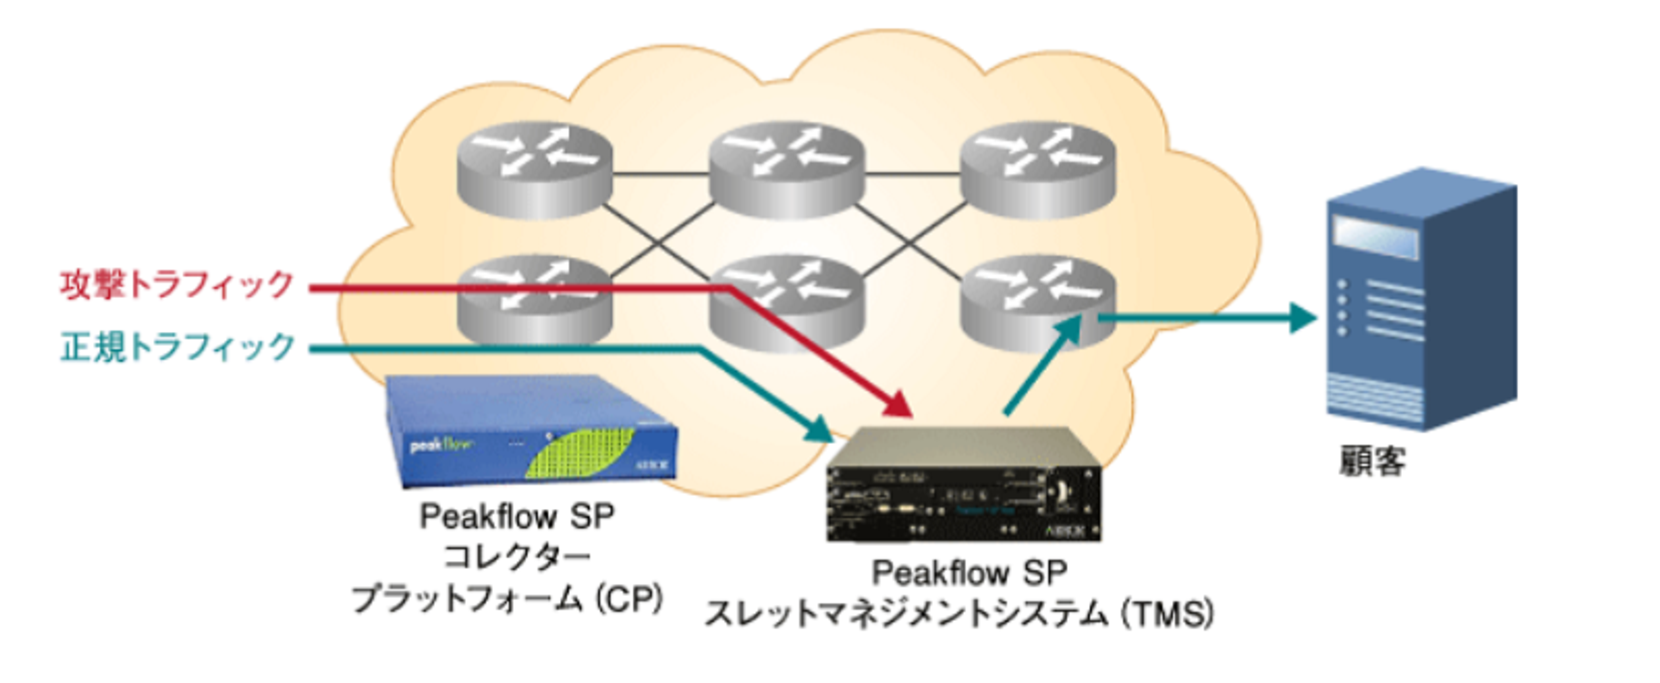
\includegraphics[height=60mm]{figures/arbor.eps}
       \caption{Arbor Networks Peakflowのシステム概要\cite{ar}}
    \label{fig:arbsys}
    \end{figure}

\subsection{Clam AntiVirus}

Clam AntiVirus\cite{ClamAV}はオープンソースで提供されているクロスプラットフォームのアンチウィルスソフトウェアである.シグネチャと呼ばれるマルウェアの特徴を記載したファイルによるパターンマッチング方式を
採用しており,約21755種類のウィルスに対応をしている.公開されているシグネチャを用いてホスト上にあるファイルをスキャンしシグネチャと一致したファイルが無いか探索を行う.シグネチャと一致するファイルがあった場合には,ユーザーに対して通知を行う.
